\section{Detection Strategy}\label{sec:detection}

The identification of these type-aware practices is implemented in three components, which is illustrated in Figure \ref{fig:components}.

\noindent\textbf{\emph{AST Parser.}} The component first extracts all Python files from the analyzed system and parses them into Abstract Syntax Trees (AST). ``Assign Stmt Entities'' (i.e., Assignment Statement Entities), ``Call Expr Entities'' (i.e., Call Expression Entities) and ``Delete Stmt Entities'' (i.e., Delete Statement Entities) in parsed ASTs are stored to be further analyzed for detecting the studied practices.

\noindent\textbf{\emph{Type Analyzer.}} The key of detecting type inconsistencies is type inference for Python programs. Type inference for dynamically typed languages is highly challenging, thus general type inference techniques fail in a small part of variables \cite{b14}. Therefore, we combine the results of Pysonar2\cite{b41} and Mypy\cite{b42} to determine the types of all variables and arguments in the analyzed system, where Pysonar2 is a widely-used type inference tool for Python code and Mypy is a static type checker for Python code. Although Mypy is mainly used to find common type-related errors by combining the benefits of dynamic typing and static typing, it contains a powerful type system thus we utilize its limited type inference feature to infer data types. During the detection of the studied practices, when Pysonar2 fails to infer the type of a variable or an argument, then we refer to the help of Mypy.

\noindent\textbf{\emph{Practice Detector.}} Based on the extracted AST entities and the inferred types in the system, this component detects the occurrences of dynamic type-aware practices by checking type inconsistencies and analyzing AST nodes. The detection condition of each studied practice is listed as follows:
\begin{itemize}
	\item 
	\emph{Inconsistent Assignment Types}: for the defined variable $v$ in each of Assign Stmt Entities,  the types of $v$ before and after the assignment are inconsistent types.
	\item 
	\emph{Inconsistent Argument Types}: for each formal parameter $p$ in each method $m$, the types of argument values of $p$  in Call Expr Entities which call $m$ are inconsistent types.
	\item 
	\emph{Inconsistent Variable Types}: for each used variable $v$ in AST entities, the types of $v$ following different execution are inconsistent types.
	\item 
	\emph{Dynamic Element Deletion}: for each entity $e$ in Delete Stmt Entities, one of the deletion targets is an instance of ``\textit{Subscript}''.
	\item 
	\emph{Dynamic Attribute Deletion}: for each entity $e$ in Delete Stmt Entities, one of the deletion targets is an instance of ``\textit{Attribute}''; or for each entity $e$ in Call Expr Entities, the function name of $e$ is ``\textit{delattr}'' and the type of the second argument is \textit{string}.
	\item 
	\emph{Dynamic Attribute Access}: for each entity $e$ in Call Expr Entities, the function name of $e$ is ``\textit{getattr}'' and the type of the second argument is \textit{string}.
\end{itemize}

\begin{figure}
	\centering
	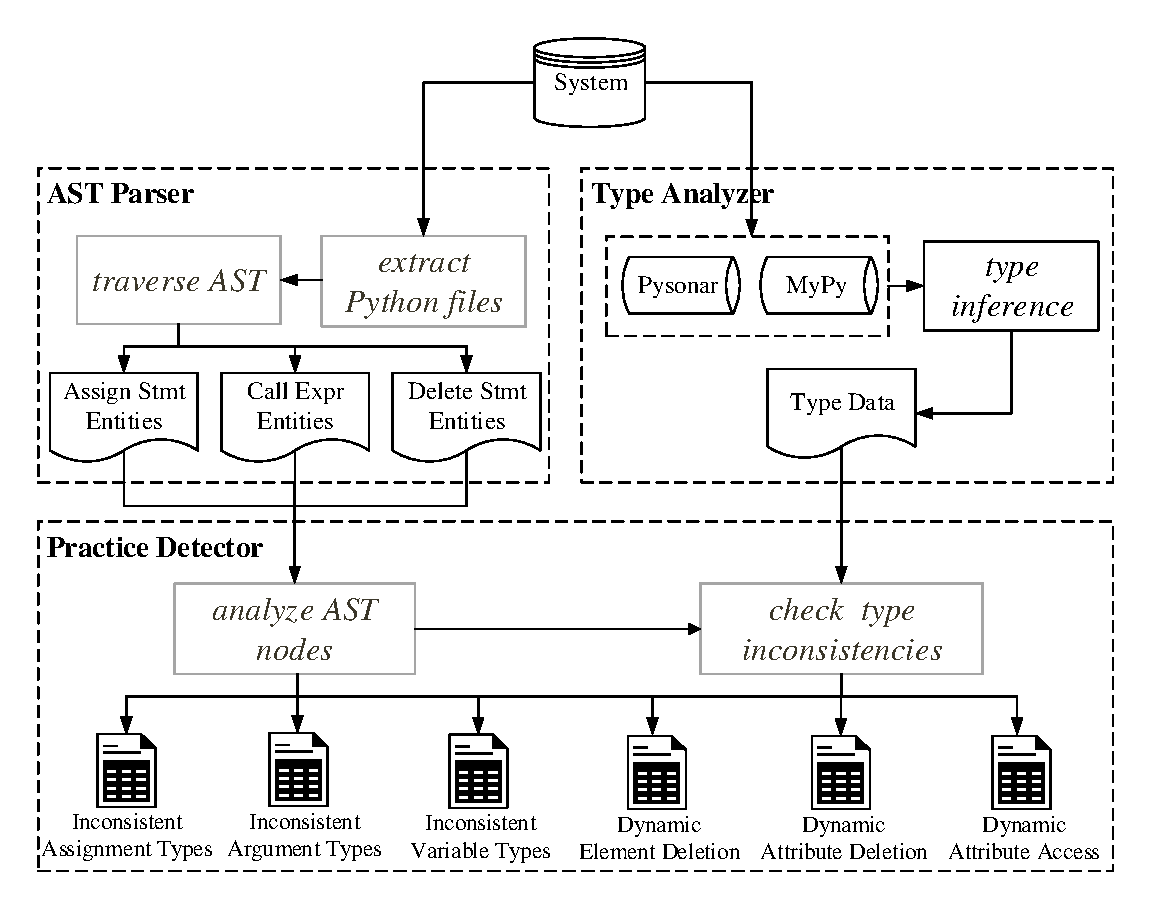
\includegraphics[width=1.0\linewidth]{figures/components.pdf}\vspace{-10pt}
	\caption{Identification of Dynamic Type-Aware Practices}\label{fig:components}
\end{figure}